\section{Models and Methods}
\label{sec:methods}

We consider the problem of sequencing a single long DNA molecule (e.g. a chromosome) using linked reads. 
We first introduce the notion of barcode graph, discuss its link with well-known graph classes leading to the conclusion that solving the molecules ordering problem for a barcode graph is likely difficult. 
Next we introduce another graph structure, the local clique-pairs graph, inspired of approaches used to realise an interval graph.

We assume that the sequencing data were obtained by sequencing $n$ fragments (called \textit{molecules} from now) from the chromosome, each molecule being assigned a barcode, where several molecules can be assigned the same barcode; for a molecule $m$ we denote by $b(m)$ its barcode.
We denote by $\Balph{}$ the barcode alphabet and by $|\Balph|=m$ its size, i.e. the total number of observed barcodes; for a barcode $b$ we denote by $m(b)$ the molecules it labels (the barcode size). Let $F = \max_{b\in \Balph} |m(b)|$.
Finally, we assume that no two molecules do start at the same coordinate, which implies that molecules can be totally ordered by their start coordinates.

% -----------------------------------------------------------------------------------------
\subsection{Barcode graphs and families of interval graphs. \label{sec:interval_graph}}
\label{ssec:barcode_graphs}

The sequenced molecules can be seen as intervals along the real line if the sequenced chromosome is linear, or arcs around a circle if it is circular; their \textit{intersection graph} is the graph whose vertices are the $n$ molecules and two vertices are linked by an edge if the corresponding intervals do intersect. 
Intersection graphs of intervals on the real line (resp. arcs around a circle) form the class of \textit{interval graphs} (resp. \textit{circular-arc graphs}).
It is well-known that deciding if a graph is an interval graph or an arc-circular graph can be done in linear time~\cite{BoothL_1976,McConnell_2003}, and many algorithmic problems that are computationally hard in general graphs are tractable in these graph classes~\cite{Golumbic_2004}.

However, the result of the sequencing experiment with linked reads does not provide direct knowledge of the sequenced molecules and of their intersections, as the reads originating from molecules having the same barcode $b$ are all labeled by $b$ and, as discussed in introduction, the problem of separating reads with the same barcodes into cluster corresponding to molecules is non-trivial.
Nevertheless, we assume here first that it is possible to infer, from the barcoded reads if, for a given pair of barcodes $b_1,b_2$ there exists molecules  $m_1$ and $m_2$ such that $b(m_1)=b_1$, $b(m_2)=b_2$ and  and $m_1$ and $m_2$ do intersect: we then say that barcodes $b_1$ and $b_2$ do \textit{intersect}. 
We assume here moreover that we do not observe two intersecting molecules $m_1$ and $m_2$ such that $b(m_1)=b(m_2)$\footnote{We justify this assumption as such molecules could be seen as a single molecule defined by the union of $m_1$ and $m_2$; moreover, simulations with realistic sequencing parameters show that this situation occurs rarely and most often with molecules that share a small intersection.}.

\begin{definition}
    \label{def:barcode_graph}
    The \textit{exact barcode graph} of a set of barcoded molecules is the graph with vertex set $\Balph{}$ and edges between pairs of intersecting barcodes. 
\end{definition}

In the case of a linear chromosome, exact barcode graphs generalize the class of interval graphs and form another well-studied graphs class, \textit{multiple-interval graphs}~\cite{FellowsHRV_2009}. 
Moreover if we assume that each barcode labels exactly $f$ molecules, exact  barcode graphs form the class of $f$-interval graphs; finally, under the additional assumption that all sequenced molecules have exactly the same length, exact barcode graphs are equivalent to the class of \textit{unit $f$-interval graph}. 
We are not aware of any study of the equivalent graph classes for circular chromosomes, i.e. arcs around a circle, and from now on we concentrate on the case of linear chromosomes.
We describe below the formulation of several algorithmic problems related to barcode graphs and how they translate into problems on the aforementioned graph classes.
Note that an exact barcode graph can be a multi-graph in the case where there exists molecules $m_1,m_2,m_3,m_4$ with $b(m_1)=b(m_3)$, $b(m_2)=b(m_4)$ and $m_1,m_2$ (resp. $m_3,m_4$) do intersect.

\smallskip\noindent\textit{Recognizing exact barcode graphs.}
The link with unit $f$-interval graph, although it assumes an unrealistic uniformity in the sequencing process (uniform molecules length and uniform number of molecules per barcode) sheds a light on the computational hardness of analyzing barcoded sequencing data. 
Indeed, recognizing $2$-interval graphs is NP-complete~\cite{WestS_1984}, while the complexity of recognizing unit $f$-interval graphs is still open,  the only positive recognition result being for depth-2 unit $f$-interval graphs~\cite{Jiang_2013}, corresponding to the case where no chromosome base is covered by more than two molecules, an unrealistic assumption for sequencing experiments. 
To the best of our knowledge, given a graph on a barcode alphabet whose edges represent possible molecules intersections, deciding if it is an exact barcode graph, even in the setting of molecules of uniform length and barcodes of uniform size, is open.

%Also, many optimization problems are tractable in interval graphs but intractable in multiple-interval graphs~\cite{ButmanHLR_2007,FellowsHRV_2009}.
\smallskip\noindent\textit{Realizing an exact barcode graph.}
A barcode sequence is a sequence $b_1 \dots b_n$ over the barcode alphabet. 
Given a barcode graph $BG$, a barcode sequence \textit{realizes} $BG$ if every edge of $BG$ can be assigned to two barcodes of the sequence in such a way that if $b_j$ is covered by an edge between $b_i$ and $b_k$ (i.e. $i<j<k$) then there are also edges between $b_i$ and $b_j$ and between $b_j$ and $b_k$.
The molecules ordering problem applied to an exact barcode graph $BG$ is then equivalent to finding a barcode sequence realizing $BG$. 
This problem is tractable in the case of interval graphs ($F=1$); note that if intervals lengths are also fixed, then the problem becomes NP-complete~\cite{PeerS_1997}, while it solvable in polynomial time if additionally the intersection lengths are provided~\cite{KoblerKW_2015}.
We are not aware of similar tractability results for multiple-interval graphs.
However, existing algorithms to realize interval graphs are mainly based on the property that such a realization can be obtained by a sequence of overlapping maximal cliques.
While maximal cliques are easy to find in an interval graph, it is not the case in multiple-interval graph, as the problem of finding the maximum clique in multiple-interval graphs is NP-complete, even for unit $2$-interval graphs~\cite{FrancisGO_2015}, although approximation and parameterized algorithms do exist~\cite{ButmanHLR_2007,FellowsHRV_2009}.
Moreover a structural property of interval graphs that is important toward the realization through maximal cliques, the existence of a vertex whose neighborhood is a clique, does not hold for multiple interval graphs~\cite{Bar-YehudaHNSS_2006}.
Finally, it is easy to see that a maximal cliques of size $c$ in an exact barcode graph might not correspond to a set of $c$ pairwise intersecting molecules.
This leads us to conjecture that realizing an exact barcode graph is difficult.

\smallskip\noindent\textit{Handling inexact barcode graphs.}
Constructing an exact barcode graph implies to detect intersecting barcodes from sequenced barcoded reads and it is thus likely unrealistic to expect perfectly obtaining such a graph from sequencing data. 
It follows that solving the molecules ordering problem would then implicitly assumes to solve a graph modification problem, aimed at transforming  a graph into a multiple-interval graph, with additional constraints about the number of occurrences of barcodes in a realization.
Graph modification problems that aim to minimize the number of modifications are generally hard, even in the case of interval graph,~\cite{CrespelleDFG_2020}, and so for multiple-interval graphs; note however that it was recently shown to be fixed-parameter tractable~\cite{VillangerHPT_2009,BliznetsFPP_2018,CrespelleDFG_2020}.
Such problems naturally translates into vertex ordering optimization problems (also known as graph layout problems) that can, in principle, be addressed with combinatorial optimization techniques such as Integer Linear Programming (ILP).
However, ILP approaches to vertex ordering currently do not scale to the size of instances corresponding to sequencing experiments~\cite{Coudert_2016}.

\smallskip
From the link we described above between barcode graphs and multiple-interval graphs, and the current state-of-the art in multiple-interval graphs algorithms, it does not appear that the problem of realizing a barcode graph can be addressed by existing algorithms, and we actually conjecture that this problem is difficult, whether the provided barcode graph is exact or not. 
Nevertheless, toward application to real sequencing data, additional assumptions about the sought realization, such as the expected length of intervals or the expected size of the barcodes, lead to specific open problems of interest in the field of multiple-interval graphs algorithms that deserves further research.


% % -----------------------------------------------------------------------------------------
% \subsection{Barcode graph structure}\todo{Titre \`a changer.}
% \label{ssec:repeats}
% \todo[inline]{CC. Je ne trouve pas cette section super-convaincante en fait. L'introduction de types de barcode graphs cr\'ee une confusion avec la section suivante.}
%
% It follows from the previous section that it is likely unrealistic to address the molecules counting and ordering problems from a started from a graph aimed at representing all molecules intersection.
% In this section we shift our focus and consider that we can more likely detect large intersections between molecules. 
% We say that two barcodes are $\ell$-intersecting if there exists a molecule $m_1$ of barcode $b_1$ and a molecule $m_2$ of barcode $b_2$ such that $m_1$ and $m_2$ do intersect on at least $\ell$ bases, and \textit{max-intersecting} if the intersecting molecules are consecutive in the true molecules ordering.
%
% \begin{definition}
%     \label{def:l_max_barcode_graph}
%     The \textit{$\ell$-barcode graph} (resp. max-barcode graph) of a set of barcoded molecules is the graph with vertex set $\Balph{}$ and edges between pairs of $\ell$-intersecting barcodes (resp. max-intersecting barcodes).
% \end{definition}
%
% While it might be unrealistic to expect one can construct a max-intersecting barcode graph from sequencing data, we make here the assumption that for $\ell$ large enough, the $\ell$-barcode graph might be a good approximation of the max-barcode graph. 
% We first look at properties of the max-barcode graph, assuming it is a multi-graph, i.e. that if it occurs $r$ times along the chromosomes that consecutives molecules have barcodes $b_1$ and $b_2$, then there are $r$ edges between $b_1$ and $b_2$.
%
% \begin{property}
%     \label{prop:eulerian_1}
%      The true barcode sequence\todo{Still undefined but should be defined earlier with the molecules ordering problem.} is a Eulerian walk of the max-barcode graph.
% \end{property}
%
% The property above shows that the ambiguity created by barcoding molecules leads to the same issue caused by repeats in classical assembly problems, i.e. that there are likely many different Eulerian walks of the max-barcode graph. 
% A triplets of barcodes $b_1,b_2,b_3$ is a $3$-repeat if there are two occurrences of three consecutive molecules of respective barcodes $b_1$, $b_2$ and $b_3$ in this order.
%
% \begin{property}
%     \label{prop:eulerian_2}
%      If the max-barcode graph has no $3$-repeats, then it is possible to determine the unique  Eulerian walk giving the true barcode sequence.
% \end{property}
%
% This property, whose proof is straightforward, suggests that identifying groups of barcodes associated to more than two consecutive molecules provide a signal that allows to infer the true barcode sequence, i.e. to solve the molecules ordering problem. 
% We describe in Appendix experiments on simulated data that shows that when $\ell$ increases, the number of occurrences of triplets of $\ell$-intersecting molecules having the same three barcodes decreases rapidly. 
%
% This observation motivates the introduction of a novel graph structure, called $d$-graphs, that we describe in the next section, aimed at capturing in the $\ell$-barcode graph the molecules ordering signal provided by consecutive groups of molecules, under the assumption that with $\ell$ large enough this signal will have a low level of ambiguity due to repeated configurations.

% -----------------------------------------------------------------------------------------
\subsection{The Local Clique-Pairs Graph}
\label{ssec:d_graphs}

In this section, we assume that we are given a barcode graph $BG$.  The barcode graph needs not be perfect: it might contain additional (wrong) edges that do not correspond to a true overlap between molecules of two barcodes, or even have missing edges. We will describe the construction of another graph based on the $BG$: the local clique-pairs (lcp) graph. We will then use the lcp graph to identify a sequence of barcodes that reflects the true order of molecules.

The idea behind the lcp graph will be that, similarly to interval graphs, a realization of an exact barcode graph can be described as a succession of overlapping maximal cliques. Intuitively, these maximal cliques correspond to a set of barcodes that each contain at least one molecule coming from a common genomic region. %\footnote{RC to YD and CC: I've added this sentence but feel free to modify it.}. 
The task is made more difficult by the fact that not all maximal cliques in a barcode graph satisfy this property. 
We observed that one can identify and skip such 'wrong' maximal cliques by instead considering a slightly more advanced object: pairs of co-localized maximal cliques, that we name local clique-pairs.  

\begin{definition}
    \label{def:lcp}
    Let $c$ be a vertex of a barcode graph $BG$. A local clique-pair (\textit{lcp}) is a triplet $(c;C_1,C_2)$ where $C_1$ and $C_2$ are maximal cliques in the neighborhood of $c$. If there are $k$ edges between vertices of $C_1$ and vertices of $C_2$ and $d$ is the maximum number of vertices in either $C_1$ or $C_2$ ($c\leq d$), the weight of the lcp $(c,C_1,C_2)$ is  defined by $w(c;C_1,C_2)=|d(d-1)/2 - k|$.~\footnote{The weight is presented for an ideal case where no node is shared between the cliques. If $C_1$ and $C_2$ share nodes, there two modification. For each node shared, 1 is added to the weight because the shared node is due to a barcode collision. Each shared edge between $C_1$ and $C_2$ count for 2 additional points in the score instead of 1, because 2 edges can be merged inside.}
\end{definition}

The definition of the weight of an lcp follows from the following observation: when molecules are all of the same length and are evenly spaced along the chromosome, if both cliques  $C_1$ and $C_2$ are of size $d$ and do indeed correspond to the $d$ barcodes of the molecules preceding (resp. following) the molecule of barcode $c$, then one expects to observe $d(d-1)/2$ edges between them in the barcode graph. So the weight measures the divergence between the observed number of edges between $C_1$ and $C_2$ and the expected number of edges in the case of uniform sequencing (see Fig.~\ref{fig:perfect_udg}).

\begin{figure}[htp]
    \centering
    %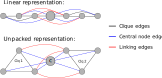
\includegraphics[width=0.7\textwidth]{lcp.pdf}
    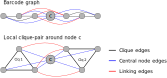
\includegraphics[width=0.7\textwidth]{lcp_2.pdf} %RC: minor cosmetic changes
    \caption{(Top) linear representation of a barcode graph obtained from $7$ molecules of uniform length. (Bottom) The local clique-pair associated to $c$. In black, the edges from the side cliques of the unit 3-graph. In blue, the edges between the central nodes and the other nodes. In red, the edges between the cliques.}
    \label{fig:perfect_udg}
\end{figure}

To motivate the introduction of lcps, we ran an experiment described in Appendix~\ref{appendix:perfectlcps}, that shows that the rate of lcps that actually encode the barcodes of consecutive molecules is higher than the rate of maximal cliques having the same property (Table~\ref{tab:clqvslcp}).
%Table~\ref{tab:clqvslcp} shows that the proportion of perfect lcps (13.5-50\%) is higher than the proportion of maximal cliques (8-9\%) in synthetic barcode graphs, motivating the use of lcps instead of maximal cliques for realizing barcode graphs.

We now discuss our algorithm to compute lcps.
Given a barcode $c$, there can be many maximal cliques among nodes in its neighborhood, especially cliques that involve the two barcodes that respectively precede and follow $c$ in the true barcode sequence.
%We do not want to keep those cliques within a lcp centered at $c$.\footnote{RC to YD: I don't understand why we don't want these cliques. Can you elaborate why? YD: I don't remind me writing that. Maybe a remnant part from older versions. I delete}
Given the set of all maximal cliques, we thus need to extract a matching defining pairs of cliques $C_1$ and $C_2$ forming lcps.
To do so, given the set of all maximal cliques in the neighborhood of $c$, we consider the complete graph whose vertices are maximal cliques and edges are putative lcps.
Let $W$ be the maximum observed lcp weight among these potential lcps. 
We replace the weight $w$ of each lcp by $W-w$ and apply a maximum-weight matching to 
clique pairs in order to obtain the set of lcps associated to $c$ (Algorithm~\ref{algo:audg}, illustrated in Fig.~\ref{fig:mwm}).

\begin{algorithm}
    \caption{Determination of a set of lcps centered at a barcode $c$.}
    \label{algo:audg}
    \begin{algorithmic}[1] % The number tells where the line numbering should start
        \Procedure{compute\_Lcp}{$c, BG$} \Comment{c: barcode, BG: barcode graph}
            \State $LCP \gets$ \O
            \State $nbs\gets BG.neighbors(n)$
            \State $subgraph \gets BG.induced\_subgraph(nbs)$
            \State $cliques \gets subgraph.max\_cliques()$ \Comment{Enumerate maximal cliques}
            \State $CG \gets clique\_graph(cliques)$ \Comment{Clique graph from divergences}
            \State $m = CG.maximum\_weight\_matching()$
            \For{$(C_1, C_2) \in m$}
                \State $LCP \gets LCP \cup new\_lcp(c, C_1, C_2)$ \Comment{Add the new Lcp}
            \EndFor
            \State \textbf{return} $LCP$
        \EndProcedure
    \end{algorithmic}
\end{algorithm}
%\footnote{Rayan to Yoann: what are $U$ and $Lcp(x,y,z)$ in the algorithm?\\
%Y: $U$ a typo from a previous version, $LCP$ the set of all generated LCP centered on $x$.}

\begin{figure}[htp]
    \centering
    %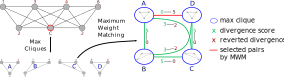
\includegraphics[width=\textwidth]{mwm.pdf}
    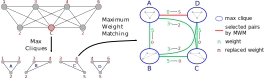
\includegraphics[width=.95\textwidth]{mwm_v2.pdf} % RC: made some cosmetic changes
    \caption{Top left: barcode graph; bottom left: max-cliques of the barcode graph; right: max-clique graph construction and maximum weight matching to construct lcps.}
    \label{fig:mwm}
\end{figure}

The time complexity of enumerating all maximal cliques of a graph is exponential~\cite{TomitaTT_2006}, while computing a maximum-weight matching is polynomial-time solvable~\cite{Galil_1986}. 
We implemented Algorithm~\ref{algo:audg} in Python using the output-sensitive cliques enumeration and maximum-weight matching methods implemented in the Networkx library~\cite{HagbergSS_2008}. Its complexity is $O(\max(C^3, M(n) C))$ with $n$ the number of graph nodes, $C$ the number of maximal cliques in the graph, and  $M(n)$ the cost of multiplying two $n\times n$ matrices.
%\footnote{CC. Est-ce qu'on peut \^etre plus or\'ecis sur le temps d'ex\'ecution?\\
% RC: oui surement.. Yoann, tu tilises \texttt{find\_cliques()} de networkx?
 %si oui, le papier cité % %https://www.sciencedirect.com/science/article/pii/S0304397508003903?via%3Dihub
 %par networkx dit: " all maximal cliques of a n vertices graph can be enumerated using $n^2$ %space, and with time delay $O(M(n))$ with $M(n)$ the cost of multiplying two n × n %matrices."\\
 %Y: D'accord avec Rayan sur le find\_cliques, puis $n^3$ pour le matching, n étant le nb de %maxcliques sorties par l'étape précédente.}
%\todo[inline]{CC. je ne suis pas s\^ur de comprendre la figure. Surtout les cliques sont disjointes, ce qui est contre-intuitif je pense. Si on cherche toutes les cliques maximales dans un voisinage on ve surement en avoir qui partage un (ou plusieurs) sommet(s).}
%\todo[inline]{Figure 2 will change according to CC's comment: Si on prend un exemple simple, 3 molecules avant c (1,2,3) et 3 molecules apres (4,5,6) espac\'ees r\'eguli\`erement, on a 4 cliques maximales, (1,2,3,c), (2,3,4,c), (3,4,5,c), (4,5,6,c) et le MWM ressort deux lcps, (c,(1,2,3),(4,5,6)) et (c,(2,3,4),(3,4,5)) et on est pass\'e de 4 cliques maximales \`a deux lcps. Mais il est difficile de discuter de la qualit\'e d'un tel r\'esultat sans parler de comment on utilise ces lcps par la suite.}

Local search for linked cliques are akin to local graph community detection.
Soft clustering is being performed with maximal clique detection, i.e. a node may belong to multiple communities.
This property leads to a lcp detection algorithm that, intuitively, is resilient to the situation where a barcode corresponds to strictly more than 2 molecules. Yet our algorithm is not perfect: it can also generate lcps that do not reflect a collection of overlapping molecules (due to additional artifactual maximal cliques); and also, missing edges in the barcode graph may lead to missing lcps.

In the ideal case, lcps can be totally ordered according to their overlaps. But because of artefactual and missing lcps, a total order is not always self-evident.
By introducing the concept of lcp graph, we are creating a new structure that can reveal a large linear lcp successions and filter out lcps that are not overlapping with others.

\begin{definition}
    \label{def:lcp_graph}
    Let $BG$ be a barcode graph and $V$ a set of lcps obtained from $BG$. The lcp graph $lcp(BG)$ is the weighted graph with $V$ for vertex set and where there is an edge between two lcps $(b;B_1,B_2)$ and $(c;C_1,C_2)$ such that some barcode belongs to both one of the $C_i$ cliques and one of the $B_i$ cliques. The weight of an edge is the size of the symmetric differences of the barcodes content of $(b;B_1,B_2)$ and $(c;C_1,C_2)$. 
\end{definition}

The figure \ref{fig:deconv} highlight the linear structures revealed by the lcp graph on synthetic barcodes.

In the following, we will describe how we determine a barcode ordering based on finding a path in the lcp graph.

%\todo[inline]{CC. Mon commentaire est plut\^ot que la remarque utilise un vocabulaire impr\'ecis (resilient, multiple local merges, wrong udg, missing udg) ce quei la rend difficile \`a comprendre. C'est plus une question de reformulation, mais qui rejoint mon commentaire plus haut sur la difficult\'e d'interpr\'eter les udg/lcp en isolation d'un algorithme qui traverse le graphe.
%RC: d'accord avec la remarque de CC, qui pourrait être adressée en étant plus précis sur le 'multiple local merges' et 'wrong and others are missing': par exemple en donnant un exemple d'udg incorrect (et d'un manquant, mais je réalise que pour manquant c'est peut-être pas facile de construire un tel exemple).}


% Rayan to Cedric:  j'ai enlevé cette partie, suite à une discussion avec Yoann, qui pense que ce n'est pas toujours vrai pour 2 raisons:
% - aux bords du barcode graphe, le lcp risque de ne pas trouver le bon ordre des barcodes car il n'y aura pas de cliques
% - si basses couvertures, alors on pourrait avoir des d-graphes avec d=1 et du coup, pas vraiment de possibilité de trouver de lcp
% donc il faudrait surement définir précisément des conditions 'idéales' plus précises pour avoir le résultat que tu escomptes
%\todo[inline]{CC. Je pense que le bout de texte suivant est vrai. Ca pourrait valoir le coup de le prouver.}
%It is straightforward\todo{CC. A prouver \dots peut-\^etre difficile \`a cause des intervalles-extr\'emit\'es qui n'ont pas de lcp.}  to see that, in the case where each barcode labels exactly one molecule and $BG$ is an exact barcode graph, then $BG$ is an interval graph and one can obtain easily from the lcp graph a realisation of $BG$ which is the true barcode sequence. While this is not an optimal way to realise an interval graph due to the maximal cliques computation, this shows that the concept of lcp graph is relevant for the problem of molecules ordering.

%\todo[inline]{CC. Ma d\'efinition du poids d'une ar\^ete est peut-\^etre fausse. Elle correspond \`a mon interpr\'etation de sommet extr\^eme, mais je ne suis pas s\^ur d'avoir compris.} % Yoann a dit que c'est OK

%\todo[inline]{CC. Pr\'esent\'e comme cela, sans exemples, j'ai peur qu'un arbitre puisse penser qu'on a cr\'e\'e une structure qui est en fait plus lourde que le barcode graph et difficile \`a analyser. Il faut soit des exemples visuels qui montrent que ce graph est plus lin\`eaire qu'un barcode graph, soit un algorithme de layout avec des r\'esultats.}


% ancien texte a cette section:
%TODO: Voir avec Rayan pour utilisation threshold/moyen plus malin.
%Interesting assembly properties.
%Cedric work on path retrieving ?\todo{Non car je n'ai pas de r\'esultats \`a montrer.}
%conclusion: More interesting solution for counting problem (filter out a lot of wrong udgs).
%Assembly process allow to traverse the graph and try to extract total order.

\begin{figure}
\includegraphics[height=4cm]{figs/simu_0_bar_n10000_d10_m3-dev1.gexf.png}\hspace{1cm}
\includegraphics[height=4cm]{figs/simu_0_bar_n10000_d10_m3-dev1_d2_simplified_maxclq-cropped.pdf}\hspace{1cm}
    \centering
    %\includegraphics{}
    \caption{Left: barcode graph of a simulated interval graph, 3k nodes and 98k edges. Right: Resulting lcp graph, 13k nodes and 23k edges. (Gephi, ForceAtlas 2 layout~\cite{gephi})}
    \label{fig:deconv}
\end{figure}


\subsection{Finding a suitable path in the lcp graph \label{sec:suitable_path}}

Recall that the molecule counting problem amounts to finding how many molecules were merged in each barcode. The molecule ordering problem asks for a sequence of barcodes that reflecst the order of molecules. As these two problems are centered on barcodes, we need a way to convert a lcp path into an ordered list of barcodes.  We do this as follws: each lcp in the path is replaced by its central barcode. %This simplification is a good proxy to approximate the barcode succession instead of the lcp succession.

Figure \ref{fig:deconv} illustrates that the lcp graph constructed from a synthetic barcode graph has a visibly linear structure. This makes the task of finding a suitable path within the lcp graph that reflects the ordering of molecules easier than in the barcode graph. 
To do this, we perform two steps: i) edge reduction within the lcp graph to remove redundant edges, and ii) a greedy algorithm with local branch and bound refinements which finds an initial path and improves it.

\paragraph*{lcp graph simplification} We simplify the lcp graph by performing transitive reduction over triplets.
Given an edge $(a,b)$ of weight $w_{ab}$, we remove this edge from the graph if there exist 2 edges $(a,c)$ of weight $w_{ac}$ and $(b,c)$ of weight $w_{bc}$ such that $w_{ab} \leqslant w_{ac} + w_{bc}$.
This operation does not change the node set (lcps) but reduces the number of possible paths to explore.
Intuitively, requiring to go through lcp $c$ when going from lcp $a$ to lcp $b$ forces to select two higher-confidence lcp overlaps instead of one lower-confidence lcp overlap.

\paragraph*{lcp path construction}

Assuming the barcode graph has been obtained by merging nodes of the exact interval graph defined by the molecules intersections, every edge of the barcode graph does correspond to one (or potentially several) edges of this interval graph; we show in Section~\ref{sec:bg_reads} that barcode graphs created from reads have nearly all correct edges corresponding to such molecules intersections.
%Toward solving the problem of computing a walk in the lcp graph that reflects the true order of molecules, this observation motivates to require that such a walk should be composed of lcps that contain most of the edges of the original barcode graph.
This observation motivates to require that a walk in the lcp graph that reflects the true order of molecules should be composed of lcps that contain most of the edges of the original barcode graph.
We define a \textit{covering variable} $v_i$ for each edge $e_i$ of the barcode graph.
Each lcp is an induced subgraph of the barcode graph, so it can be associated to a set of covering variables, i.e. edges of the barcode graph.
We will seek a path such that the union of covering variables over all its constituent lcps is as close as possible to the set of all covering variables.%\footnote{RC to YD: better?}

Our lcp path construction strategy is a local branch \& bound algorithm.
Assuming we have already constructed a path of lcps $p = l_1,\ldots,l_i$, we consider as candidates for $l_{i+1}$ all the neighbors of $l_i$ in the lcp graph such that $l_{i+1}  \notin p$.
Those neighbors are sorted by priority over three criteria: first if one or more lcp(s) cover at least one uncovered variable, i.e. one edge of the original barcode graph, we restrict our choice to those lcps. \footnote{RC to YD: it seems that this first criterion isn't about sorting but rather removal of some candidate lcps. Is that true or did I make a mistake when rewriting that part? YD: They are not completely removed. We try first the paths with the node that come first in the sorted neighbors but the other nodes can be bridges so we try them if nothing else worked} % (otherwise, we choose the extension among all neighbors of $l_i$.
For the second sorting criterion,  we sort the candidate $l_{i+1}$'s by increasing clique pair weight. %\footnote{RC to YD: you mean lcp graph weight? YD:    No, lcp divergence. It has been recently renamed the weight of the clique pair}.
Last, if multiple candidates have equal clique pair weights, we sort them by increasing $l_i \rightarrow l_{i+1}$ edge weight in the lcp graph.
Selecting the first element in the sorted neighbors at each step defines a greedy heuristic for the path computation.

The above algorithm might result in a short path due to tips in the lcp graph, i.e. nodes of degree $1$.
In order to address this issue, we use a local branch and bound algorithm and backtrack a few nodes when a dead end is reached.
This can result in several paths and we use the number of covering variables in the path as a score to keep only the best solutions according to that score.

The last part of the algorithm is the selection of the first node $l_1$ of the path.
Because we do not have good selection criteria, we initially select a $l_1$ at random among all lcps.
We start by computing a path using the above algorithm which ends at some node $l_e$.
We then discard this part and restart again our algorithm from $l'_1 = l_e$ to create a new path, where $l_e$ has a higher chance to be an endpoint of the true lcp path than $l_1$.

%\todo[inline]{CC: I do not understand as from my understanding of the part above, $n_e$ is a dead-end.\\
%YD: Yes but we hope that it's the farthest reachable node.
%RC: I reformulated that part. }

We will show in the next section that despite this heuristic being very simple and likely leaving  room for improvement, it does work very well on simulated data, suggesting the lcp graph does actually capture a very robust signal toward recovering the correct barcode sequence.

%Of course, this heuristic is not perfect and will not always find a perfect solution. But it is sufficient to prove that retrieving a good path from our lcp graph is feasible, even with naive algorithms.


%\paragraph*{Counting molecules in path}

%%%%%%%%%%%%%%%%%%%%%%%%%%%%%%%%%%%%%%%%%%%%%%%%%%%%%%%%%%%%%%%%%%%%%%%%%%%
